\documentclass{beamer}
\usepackage{animate}
\usepackage{multimedia}
\usepackage[english,russian]{babel}

\usepackage{pgfpages}
\setbeameroption{show notes on second screen}
%https://tug.ctan.org/macros/latex/contrib/beamer/doc/beameruserguide.pdf

\usepackage[T2A]{fontenc}
\usepackage[utf8]{inputenc}

\setbeamertemplate{caption}[numbered]

\usetheme{CambridgeUS}
\usecolortheme{dolphin}


\title[Модель Блинна-Фонга]{Модель Блинна-Фонга}
\author[Быковских Д.А.]{Быковских Дмитрий Александрович}
\date{02.12.2023}

\begin{document}
	\begin{frame}
		\titlepage
	\end{frame}

	\begin{frame}{Введение}
		Модель освещения Фонга является простой, популярной и широко известной в компьютерной графике.

		Описание модели было представлено в следующей статье

		\href{https://users.cs.northwestern.edu/~ago820/cs395/Papers/Phong_1975.pdf}{Bui Tuong Phong  
		"Illumination for Computer Generated Pictures"~
		University of Utah (1975 г.)}
		
	\end{frame}

	\begin{frame}{Введение}
		В основе модели освещения Блинна-Фонга лежит алгоритм приближенного расчета интенсивности света на поверхности объектов. 
		Эта модель была предложена в 1977 году Блинном и Фонгом. 

		Один из вариантов рабочей формулы:

		\[
			I = I_a k_a + \sum_{j=1}^{m} \frac{I_{l_j}}{d+k} \bigg[ k_d (n_j \cdot L_j) + k_s (R_j \cdot v)^n \bigg]
		% ,
		\]
		% где
		% $m$ --- количество ИС.



		\note{
			Состоит из следующих частей:
			\begin{itemize}
				\item Источник света (ИС) $I_{l_j}$;
				\begin{itemize}
					\item Интенсивность излучения $I$;
					\item Функция радиального затухания $\frac{1}{d+k}$;
				\end{itemize}
				\item Свойства поверхности $k_a, k_d, k_s$;
				\begin{itemize}
					\item Фоновое освещение $I_a$;
					\item Диффузное рассеивание $(n_j \cdot L_j)$;
					\item Зеркальное рассеивание $(R_j \cdot v)^n$.
				\end{itemize}

			\end{itemize}

			Комбинация этих компонентов позволяет создавать более реалистичные изображения трехмерных объектов с учетом их взаимодействия с источниками света. 
		}

	\end{frame}






	\begin{frame}{Источники света (ИС)}
		ИС --- любой объект, излучающий энергию. \\
		Типы источников света:
		\begin{itemize}
			\item Источники направленного света;
			\item Точечные ИС;
			\item Прожекторы.
		\end{itemize}


		% \[
		% \begin{pmatrix}
		% 	Параметры
		% \end{pmatrix}	
		% \]

	\end{frame}

	\begin{frame}{Интенсивность излучения}

		Интенсивность излучения - это физическая величина, характеризующая мощность электромагнитного излучения (например, света) в определенном направлении от источника. 
		
		Она измеряется в ваттах на квадратный метр (Вт/м²).

		Математически интенсивность излучения ($I$) может быть выражена с использованием формулы:
		\[
			I= \frac{P}{A}
			,
		\]
		где
    % $I$ --- интенсивность излучения,
    $P$ --- мощность излучения (в ваттах),
    $A$ --- площадь, через которую проходит излучение (в м²).
		
		
		\note{
			Значение для каждой компоненты цвета считается независимо, т.е. $I = (I_r, I_g, I_b)$.
			
			Суммарное освещение
			\[
				I = k_e + k_a I_{a} + \sum_j I_j
			,
			\]
			где 
			$k_e$ --- способность материала излучать свет;
			$k_a I_{a}$ --- глобальную фоновую освещенность сцены;
			$I_j$ --- вклад вносимый $j$-м ИС.
			}

		\note{

		}

	\end{frame}

	\begin{frame}{Источники направленного света}
		Направленные световые источники (Directional Lights): Это источники света, которые моделируют бесконечно удаленный источник света, такой как солнце. Лучи света параллельны друг другу и идут в определенном направлении. Они используются для создания резких теней и подчеркивания форм объектов.

		\note{
			\begin{figure} 
				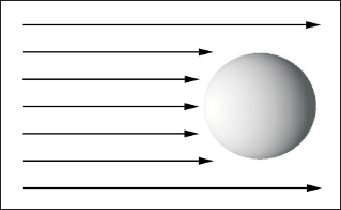
\includegraphics[width=0.75\textwidth]{images/f05_05.jpg}
			\caption{Источник направленного света}
		\end{figure}
		}
		
	\end{frame}
	
	\begin{frame}{Точечные ИС}
		Спот-свет (Spotlights): Эти источники света создают конус света, направленный в определенном направлении. Они эффективны для выделения конкретных объектов или областей в сцене. Спот-свет может имитировать направленные лучи фар автомобилей или прожекторы на сцене.

		\note{
			\begin{figure} 
				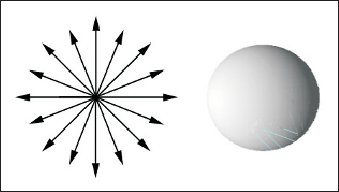
\includegraphics[width=0.85\textwidth]{images/f05_04.jpg}
			\caption{Точечный ИС}
		\end{figure}
		}
	\end{frame}

	\begin{frame}{Амплитуда затухания}

    Затухание (Attenuation): Учитывает затухание света с увеличением расстояния между источником света и поверхностью.

		Чем дальше расположен объект от ИС, тем слабее интенсивность света на поверхности 
		этого объекта.
		
		Амплитуда затухания определяется функцией радиального затухания:
		\[
			f(d_l) \sim \frac{1}{d_l^2}
			,
		\]
		где $d_l$ --- расстояние от объекта до ИС.

		Но на практике применяют следующую функцию

		\[
			f(d_l) = 
			\begin{cases}
			\frac{1}{a_0+a_1 d_l + a_2 d_l^2}, \text{для локальных ИС} \\	
			1, \text{для бесконечно-удаленных ИС} \\	
			\end{cases}	
		\]

	\end{frame}
	
	\begin{frame}{Прожекторы}
		Прожекторы (Projectors): Прожекторы в компьютерной графике используются для проецирования текстур или изображений на поверхности объектов в сцене. Они также могут быть настроены на создание направленного света в определенных направлениях.

		\[
			f(\phi) = \bigg[ \frac{(v_o, v_l)}{|v_o||v_l|} \bigg]^{a_l}
			,
		\]
		где $0 \le \phi \le \theta$.

		\note{
			\begin{figure} 
				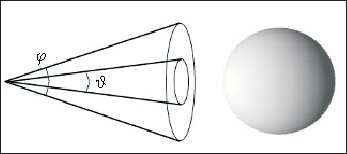
\includegraphics[width=\textwidth]{images/f05_06.jpg}
			\caption{Прожекторы}
		\end{figure}
		}
	\end{frame}


	\begin{frame}{Интенсивность углового затухания}

		Угловое затухание интенсивности --- явление, при котором интенсивность света затухает по мере увеличения угла между направлением, из которого свет падает, и нормалью к поверхности. 
		% Это явление учитывается в моделях освещения для того, чтобы объекты визуально выглядели естественно, с учетом изменения интенсивности света в зависимости от угла падения.

		Математически угловое затухание интенсивности часто выражается с использованием косинуса угла между направлением света и нормалью к поверхности. Если $\phi$ --- угол между направлением света и нормалью, то угловое затухание может быть выражено следующим образом:
		\[
			f(\phi) = \cos^{a_l} \phi
		\]


		Здесь представляет собой коэффициент углового затухания, который уменьшает интенсивность света по мере увеличения угла. Когда свет падает под прямым углом (угол), угловое затухание равно 1, и свет не затухает. При увеличении угла, значение косинуса уменьшается, что приводит к уменьшению интенсивности света.

		\note{
			\begin{figure} 
				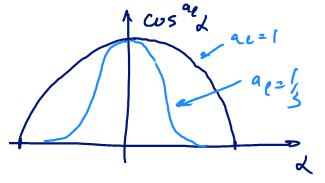
\includegraphics[width=0.75\textwidth]{images/угловое-затухание.png}
			\caption{Интенсивность углового затухания в зависимости от $a_l$}
		\end{figure}
		}
		
	\end{frame}



	\begin{frame}{Эффекты освещения поверхности}
		В компьютерной графике эффекты освещения поверхности важны для создания реалистичных и привлекательных визуальных изображений. Эти эффекты обусловлены взаимодействием света с материалами поверхности объектов. Вот несколько основных эффектов освещения поверхности:

		\begin{itemize}
			\item Фоновое освещение (Ambient Occlusion, $K_a$);
			\item Рассеянное освещение (Diffuse Lighting, $K_d$);
			\item Зеркальное отражение (Specular Reflection, $K_s$);
			\item Отраженный свет (Reflection);
			\item Преломление (Refraction);
			\item Тени (Shadows);
			\item Глосс (Gloss).
		\end{itemize}
		
		\note{
			{
			% Ambient Occlusion (AO): Этот эффект моделирует затемнение в областях, где свет имеет ограниченный доступ. Он усиливает визуальное восприятие объемности объектов, подчеркивая скрытые участки.

			% Рассеянное освещение (Diffuse Lighting): Этот эффект характеризуется равномерным рассеиванием света в различных направлениях на поверхности объекта. Интенсивность рассеянного света зависит от угла между направлением света и нормалью к поверхности. Материалы с рассеянным освещением выглядят матовыми.

			% Зеркальное отражение (Specular Reflection): Этот эффект связан с отражением света в направлении, симметричном относительно зрителя. Зеркальное отражение создает блики на поверхности материала и придает объекту блеск. Эффект сильнее выражен у гладких и блестящих материалов.
	
			Отраженный свет (Reflection): Эффект отраженного света моделирует отражение окружающей среды на поверхности объекта. Это может включать отражение других объектов, окружения или облаков.
	
			Преломление (Refraction): Когда свет проходит через прозрачные материалы, происходит преломление. Этот эффект приводит к изменению направления света и созданию искажений на границе между материалами с разными оптическими свойствами.
	
			Тени (Shadows): Тени создаются благодаря препятствиям, которые мешают свету достигнуть определенных областей поверхности. Тени важны для добавления глубины и реализма в изображения.
	
	
			Глосс (Gloss): Этот эффект описывает степень блеска или матовости поверхности. Гладкие и блестящие поверхности имеют низкую степень матовости, в то время как матовые материалы выглядят более матовыми.
			}
		}


	\end{frame}

	\begin{frame}{Свойства материала}
		Когда речь идет о свойствах материала в приложении к освещению, то имеется в виду его способность воспринимать каждую из трех компонент цвета каждой составляющей освещенности. Дополнительно, материал может сам излучать свет. Т.о. цветовые свойства материала задаются коэффициентами, которые объединяются в тройки: \\
		$k_a$ --- свойство материала воспринимать фоновое освещение; \\
		$k_d$ --- свойство материала воспринимать рассеянное освещение; \\
		$k_s$ --- свойство материала воспринимать зеркальное освещение.
		
		\note{
			К свойствам материала добавляются еще коэффициенты: \\
			$k_e$ --- свойство материала излучать свет; \\
			$k_{\alpha}$ --- прозрачность; \\
			$\beta$ --- коэффициент блеска. 
		}
	\end{frame}




	\begin{frame}{Вычисление угла между отраженным лучом и направлением на наблюдателя}
		Угол между отраженным лучом и направлением на наблюдателя можно рассчитать по следующей формуле:

		\[
			R + L=2(N \cdot L) N	
		\]
		\[
			R = 2 (N \cdot L) N - L
		\]

		Скалярное произведение $(R \cdot V)$ рассчитывается по формуле:

		\[
			(R \cdot V) =2({N}\cdot{L})({N}\cdot{V})-({L}\cdot{V})
		\]

		\note{
			\begin{figure} 
				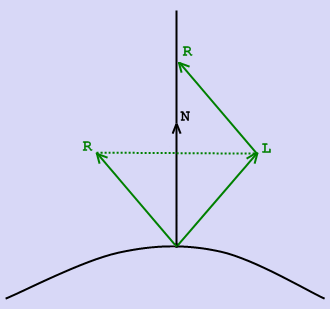
\includegraphics[width=0.5\textwidth]{images/reflect_vector.png}
			\caption{Векторы в модели освещенности Блинна}
		\end{figure}

		}

	\end{frame}




	\begin{frame}{Фоновое освещение}
		\[
			I_a = k_a I_a
			,
		\]
		где 
		$I_a$ --- фоновая составляющая освещенности в точке;
		$k_a$ --- свойство материала воспринимать фоновое освещение;
		$I_a$ --- мощность фонового освещения.

		фоновая составляющая освещенности не зависит от пространственных координат освещаемой точки и источника. Поэтому при моделировании освещения, в большинстве случае, не имеет смысла брать более одного фонового источника света. Часто просто задается некое глобальное фоновое освещение всей сцены.
		\note{
			\begin{figure} 
				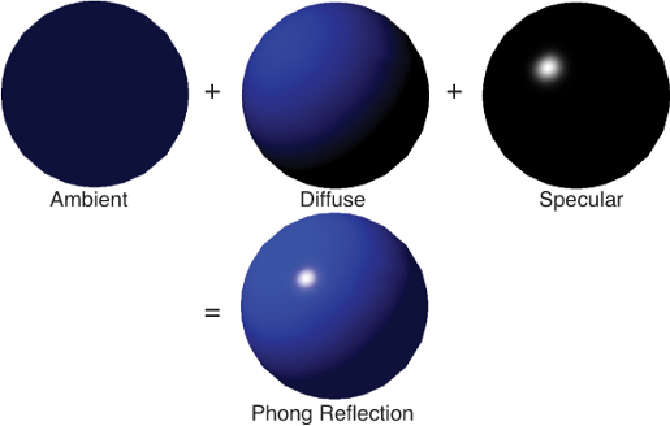
\includegraphics[width=0.75\textwidth]{images/img-gen171.png}
				\caption{Виды отражений}
			\end{figure}
		}
	\end{frame}

	\begin{frame}{Рассеянный свет}	

		Рассеянное освещение (Diffuse Reflection): Описывает равномерное рассеивание света от поверхности во всех направлениях. Интенсивность рассеянного света зависит от угла между нормалью к поверхности и направлением света.
		\[
			I_d %= k_d \cos (L \cdot N) I_d 
			= k_d (L \cdot N) I_d
			,	
		\]
		где 
		$I_d$ --- рассеянная составляющая освещенности в точке;
		$k_d$ --- свойство материала воспринимать рассеянное освещение;
		$I_d$ --- мощность рассеянного освещения;
		$L$ --- направление из точки на источник;
		$N$ --- вектор нормали в точке.
	
		\note{
			\begin{figure} 
				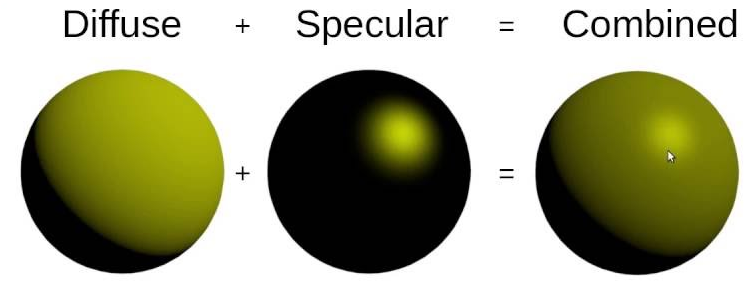
\includegraphics[width=0.75\textwidth]{images/diffuse_specular.png}
				\caption{Виды отражений}
			\end{figure}
		}

	\end{frame}

	% \begin{frame}{Рассеянное освещение}
	% 	Рассеянное освещение --- это один из компонентов модели освещения, используемый для приближенного моделирования того, как свет рассеивается на матовых поверхностях. Оно описывает явление равномерного рассеивания света во всех направлениях от поверхности.

	% 	Основная идея рассеянного освещения заключается в том, что поверхность, на которую падает свет, диффузно рассеивает его во все стороны. Интенсивность рассеянного света зависит от угла между направлением падающего света и нормалью к поверхности в данной точке. Чем ближе угол к 90 градусам (то есть, чем более свет падает под прямым углом к поверхности), тем интенсивнее рассеянный свет.
		
	% 	Математически это часто выражается с использованием закона Ламберта. Если NN - нормализованный вектор нормали к поверхности, LL - нормализованный вектор направления света, и IdId - интенсивность диффузного освещения, то интенсивность рассеянного света (IdiffuseIdiffuse) может быть выражена следующим образом:
		
	% 	\[
	% 		Idiffuse=Id \cdot (N \cdot L)Idiffuse = Id \cdot (N\cdot L)
	% 	\]
		
	% 	Здесь обозначает скалярное произведение векторов.
		
	% 	Рассеянное освещение вместе с другими компонентами, такими как зеркальное отражение и затухание, формирует комплексные модели освещения, используемые в компьютерной графике для создания более реалистичных изображений трехмерных сцен.
	% \end{frame}

	\begin{frame}{Зеркальное отражение}

		Зеркальное отражение (Specular Reflection): Моделирует отражение света от блестящих или гладких поверхностей. Этот компонент создает яркие блики на поверхности и зависит от угла между направлением обзора (направление, с которого наблюдается поверхность) и направлением отраженного света.

		\[
			I_s = k_s \cos^{\alpha}(R,V) I_s = k_s (R \cdot V)^{\alpha} I_s
			,	
		\]
		где
		$I_s$ --- зеркальная составляющая освещенности в точке;
		$k_s$ --- коэффициент зеркального отражения;
		$I_d$ --- мощность зеркального освещения;
		$R$ --- направление отраженного луча;
		$V$ --- направление на наблюдателя;
		$\alpha$ --- коэффициент блеска, свойство материала.


		\note{
			Именно зеркальное отражение представляет наибольший интерес, но в то же время его расчет требует больших вычислительных затрат. При фиксированном положении поверхности относительно источников света фоновая и рассеянные составляющие освещения могут быть просчитаны единожды для всей сцены, т.к. их значение не зависит от направления взгляда. С зеркальной составляющей этот фокус не сработает и придется пересчитывать её каждый раз, когда взгляд меняет свое направление.

			Во всех вычислениях выше, для рассеянной и зеркальной компонент, если скалярное произведение в правой части меньше нуля, то соответствующая компонента освещенности полагается равной нулю.
		}
	\end{frame}

% 	\begin{frame}{Зеркальное отражение}
% 		Зеркальное освещение — это компонент модели освещения, который моделирует отражение света от блестящих или гладких поверхностей. Этот компонент отвечает за появление на поверхности ярких бликов, которые образуются при отражении света в определенном направлении.

% Основные характеристики зеркального отражения включают в себя:

%     Отражательный вектор (Reflectance Vector): Он представляет собой направление, в котором свет отражается от поверхности. Для вычисления отражательного вектора используется зеркальное отражение относительно нормали к поверхности.

%     Блеск (Specular Highlight): Это яркое пятно на поверхности, которое возникает в результате зеркального отражения света. Чем ближе угол между направлением обзора (точка, с которой мы смотрим на объект) и отражательным вектором к 0 градусам, тем более ярким будет блеск.

% 		Математически зеркальное отражение часто описывается с использованием модели Фонга или модели Блинна-Фонга. Для данной точки на поверхности с нормалью NN, вектором направления света LL, вектором обзора VV и коэффициентом блеска ksks, интенсивность зеркального отражения (IspecularIspecular) может быть выражена следующим образом:

% 		\[
% 			Ispecular=ks \cdot (R \cdot V)nIspecular=ks\cdot (R\cdot V)n
% 		\]

% 		где RR - отражательный вектор, VV - вектор обзора, и nn - экспоненциальный коэффициент, который определяет степень блеска.

% 		Зеркальное освещение вместе с другими компонентами, такими как рассеянное освещение и затухание, входит в состав моделей освещения, используемых в компьютерной графике для достижения более реалистичных эффектов.
% 	\end{frame}


	\begin{frame}{Модель освещения и методы затенения}
		\[
			I = k_e + I_a k_a + \sum_{j=1}^{m} \frac{I_{l_j}}{d+k} \bigg[ k_d (n_j \cdot L_j) + k_s (R_j \cdot v)^\alpha \bigg]
		,
		\]
		где
		$I$ --- интенсивность излучения;
		$k_e$ --- способность материала излучать свет;
		$I_a$ --- интенсивность поглощения (absorption coefficient);
		$k_a$ --- коэффициент поглощения;
		$I_{l_j}$ --- интенсивность ИС;
		$d$ --- расстояние от ИС до объекта;
		$k$ --- константана (трюк, чем ближе, тем больше величина);
		$k_d$ --- коэффициент диффузного отражения;
		$k_s$ --- коэффициент зеркального отражения;
		$\alpha$ --- коэффициент блеска, свойство материала;
		$n_j$ --- нормаль;
		$L_j$ --- вектор направления на ИС;
		$R_j$ --- вектор отражения ИС;
		$v$ --- вектор направления камеры или точки обзора;
		$m$ --- количество ИС.

		Сравнение простейших методов затенения:

		В методе плоского затенения освещение вычисляется один раз для каждого полигона в сцене.

		В методе затенения по Фонгу для каждой вершины полигона вычисляются значения нормали и освещенности. Затем значения этих характеристик интерполируются между вершинами, чтобы получить плавное изменение освещенности на всей поверхности полигона.



		
		\note{
			\begin{figure} 
				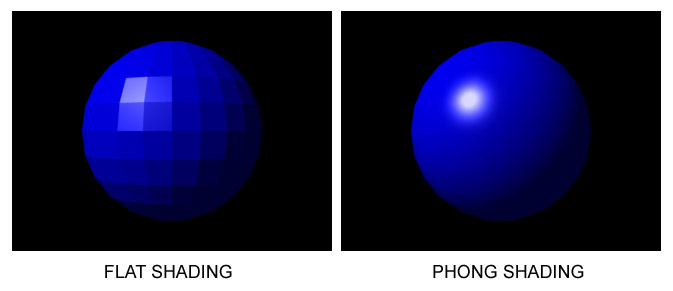
\includegraphics[width=\textwidth]{images/7UNuF.jpg}
			\caption{Сравнение плоское затенение (слева) и затенение Фонга (справа)}
		\end{figure}
		}
	\end{frame}


	\begin{frame}{Модель Блинна-Фонга}{Упрощенный расчет зеркальной компоненты освещенности}
		Для расчета отраженной компоненты требуется выполнить довольно громоздкие вычисления. Существует модель Блинна-Фонга, представляющая собой модель Фонга с упрощенным расчетом зеркального отражения. Вычислим в каждой точке вектор полупути ${H}$ (halfway vector):
		\[
			H=\frac{L+V}{|L+V|}
			,
		\]
		который показывает ориентацию площадки, на которой будет максимальное отражение. 
		\\
		Тогда величину $(R\cdot V)^\alpha$ можно заменить величиной $(H \cdot N)^\beta$.

		% При этом α <> β и, в общем случае, соотношение между ними зависит от пространственной связи векторов {V}, {L} и {N}. Вектор {H} называется вектором полупути, т.к. если все три вектора {V}, {L} и {N} лежат в одной плоскости, то угол между {H} и {N} составляет половину угла между {R} и {V}.

		% Модель отражения Блинна-Фонга никогда в точности не совпадает с моделью Фонга, однако можно подобрать соответствующие значения α и β, для которых распределения зеркальной составляющей по поверхности для обеих моделей будут очень близкими. Вместе с тем, в ряде случаев модель Блинна-Фонга требует значительно меньше вычислений, например в случае направленного бесконечно-удаленного источника.

		\note{
			\begin{figure} 
				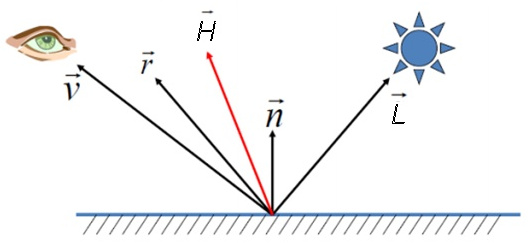
\includegraphics[width=0.75\textwidth]{images/physics_vector_blinna_fonga.jpg}
				\caption{Векторы в модели освещенности Блинна-Фонга}
			\end{figure}
			}
	\end{frame}

	\begin{frame}{Модель освещения Блинна-Фонга}
		\[
			I = K_a I_a + K_d (n \cdot l) + K_s (n \cdot h)^p
		,
		\]
		где

		$n$ --- вектор нормали к поверхности в точке;

		$l$ --- падающий луч (направление на источник света);

		$h$ --- отраженный луч (направление идеально отраженного от поверхности луча).

		\[
			h=2(l \cdot n)n-l
		,
		\]
		где

		$K_a$ --- коэффициент фонового освещения;

		$K_s$ --- коэффициент бликового освещения;

		$K_d$ --- коэффициент диффузного освещения.

		\note{
			\begin{figure} 
				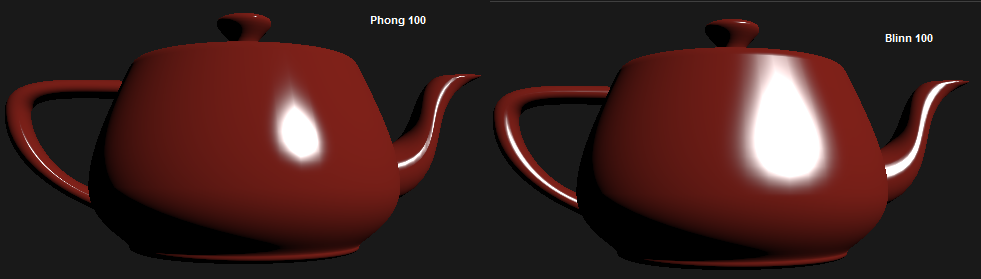
\includegraphics[width=\textwidth]{images/phong-blinn-compare.png}
			\caption{Сравнение моделей Фонга и Блинна-Фонга}
		\end{figure}
		}

	\end{frame}

	% \begin{frame}{Заключение}
	% 	Литература
	% 	\begin{enumerate}
	% 		\item \href{https://users.cs.northwestern.edu/~ago820/cs395/Papers/Phong_1975.pdf}{Bui Tuong Phong  
	% 		"Illumination for Computer Generated Pictures"~
	% 		University of Utah (1975 г.)}
	% 		\item \href{}{}
	% 	\end{enumerate}
	% \end{frame}

\end{document}
